\chapter{Evaluation}

In this chapter, we will evaluate the Psnodig tool against the goals we set in Section 1. We will look at the general effort to add a new parser, correctness and performance of our interpreter, and whether or not our writers are able to produce satisfactory output. We will also attempt to reproduce the examples in the tools introduced in Section 3, and compare it to our results. Unfortunately, only the ones relating to IBP are currently publicly available. \\

All the Psnodig examples in this chapter will be created entirely through the command line interface, to ensure that - as of writing this - all examples are reproducable. To keep a common thread going through this chapter, as well as keeping it fair to all parts of the tool, there are a few algorithms that all will be evaluated against: \texttt{Naive search}, \texttt{Bubble sort}, \texttt{Deletion in a Binary search tree} and \texttt{Depth-first search}. The results are presented in Section 6.3 and onwards. \\

On one hand, the evaluation is somewhat limited. For instance, there are almost no benchmarks that we go against. It is \textit{we} who select the computer programs, and it is \textit{we} who decide whether or not the results are adequate. \\

On the other hand, we do believe that we have chosen varied enough programs to test against. In addition, there \textit{are} some subjective standards that we can lean on, particulartly when it comes to our flowchart writer.

\subsubsection{Naive search}

Naive search is a simple algorithm where we look for a particular element in a list. It is naive because it iterates the list in a simple start-to-end fashion, without applying any heuristics, like the Binary search algorithm mentioned in Section 2.1.1.

\subsubsection{Bubble sort}

Bubble sort is one of the most straightforward sorting algorithms we have available. It is used to sort a list, making sure that for all elements, the elements on the left are smaller, and the elements on the right are bigger. Bubble sort is not used particularly often to solve real problems, and is mostly intended as a tool to teach students about sorting algorithms as a concept. \\

If the list only contains one element or is empty, we return it as it is. Otherwise, we compare the elements on index 0 and 1, and if the first is larger than the second, we swap them. Then we continue to compare the elements on index 1 and 2, and so on. We do this \texttt{n} times, where \texttt{n} equals the length of the list minus one. In each passing, the unsorted largest element in the list is placed in its proper position towards the end of the list.

\subsubsection{Deletion in a Binary search tree}

Binary search trees are common data structures in computer science. Each node has at most two child nodes, and all nodes are descendents of a single root node. Additionally, for all nodes \texttt{nd}, every node to the left of \texttt{nd} must have a value smaller than or equal to \texttt{nd}, and every node to the right must have a value greater than or equal to \texttt{nd}. \\

Deletion in a binary search tree involves finding a node with a specific value, and removing it whilst preserving the search tree's properties. There are three cases to consider: deletion of a node with no children, deletion of a node with one child, and deletion of a node with two children. \\

If a node has no children, we can simply remove it. If a node has one child, that child takes the place of its parent. If a node has two children, we substitute it with either the node with the smallest value on its right hand side, or the node with the largest value on its left hand side, before removing it.

\subsubsection{Depth-first search}

Depth-first search, also referred to as DFS, is an algorithm for traversing a graph data structure. We begin at an arbitrary node of the graph, and ``visit'' neighbouring nodes, following each path as far possible. \\

It is commonly used to identify all nodes within a connected component. If the graph we are working on is also unweighted, we can use DFS to find its shortest path.

\section{Extensibility}

The first goal of Psnodig is extensibility: we should be able to add parsers that are able to convert source code to an internal representation of Psnodig. We have successfully written a parser for an imperative, C-like programming language that we coined \textbf{Gourmet}.

\subsection{Gourmet parser}

Writing a parser on its own is no new feat, and Section 4.3 and Section 5.4.1 elaborate on the design and implementation of the Gourmet parser. What we aim to evaluate, is whether or not the parser is compatible with Psnodig. The Psnodig grammar is a limitation of how rich a program can look before it is converted by a writer. This means that a parser can at most parse all data types, but at the very least a `Program`, as it is the entry point of all Psnodig programs. \\

A minimal example is an empty program. The Gourmet parser is capable of parsing empty files, producing an AST of a single \texttt{Program Nothing [] [] Nothing} value. Since a \texttt{Program} contains \texttt{Statement}, and the latter can be compound \texttt{Statement} values, we cannot produce a maximal example.\footnote{We could interpret a maximal example to be a program limited by our computer’s memory, but theoretically Psnodig programs can be infinitely big.} \\

The Gourmet parser is built up of many smaller parsers, parsing each Psnodig data type individually. This way, we can look at it almost like a checklist, proving that we do indeed parse all Psnodig data types. \\

\Cref{naiveSearchGourmet}, \Cref{bubbleSortGourmet}, \Cref{deleteBSTGourmet}, and \Cref{dfsGourmet} show implementations of the four programs mentioned in the beginning. \\

\forsup{se på den under feks. \textbackslash in blir evaluert!}

\begin{lstlisting}[caption={Naive search implementation in Gourmet.}, captionpos=b, label={naiveSearchGourmet}]
? A list $A$ and an integer $x$?
! True if $x \in A$ and false if not!

func NaiveSearch(A list, x int) {
    # n := length(A)
    for i := A {
        if i == x {
            return true
        }
    }
    return false
}
\end{lstlisting}

\begin{lstlisting}[caption={Bubble sort implementation in Gourmet.}, captionpos=b, label={bubbleSortGourmet}]
? A list $A$?
! The list $A$, but ordered from smallest value to largest!

func BubbleSort(A list) {
    # n := length(A)
    for i := 0, n - 1 {
        for j := 0, n - i - 1 {
            if A[j] > A[j+1] {
                @{swap A[j] with A[j+1]}{
                    tmp := A[j]
                    A[j] := A[j+1]
                    A[j+1] := tmp
                }
            }
        }
    }
    return A
}
\end{lstlisting}

\begin{lstlisting}[caption={Deletion in binary search tree implementation in Gourmet.}, captionpos=b, label={deleteBSTGourmet}]
? The root node in a tree and the value of a node to be deleted?
! The updated tree with one less node!

struct Tree {
    value int,
    left Tree,
    right Tree
}

func Delete(node Tree, val int) {
    if node == nil {
        return nil
    }
    else if (node.value) < val {
        node.right := Delete(node.right, val)
        return node
    }
    else if (node.value) > val {
        node.left := Delete(node.left, val)
        return node
    }

    if (node.left) == nil {
        return node.right
    }
    else if (node.right) == nil {
        return node.left
    }

    node' := FindMax(node.left)
    node.value := node'.value
    node.left := Delete(node.left, node.value)
    return node
}

func FindMax(root Tree) {
    if (root.right) == nil {
        return (root.value)
    }

    return FindMax(root.right)
}
\end{lstlisting}

\begin{lstlisting}[caption={DFS implementation in Gourmet.}, captionpos=b, label={dfsGourmet}]
? A list of booleans, a stack of nodes, a graph and a starting node?
! The list of booleans!

func dfs(visited list, stack list, graph list, node int) {
    visited[node] := true
    append(node, stack)

    while length(stack) > 0 {
        m := pop(stack)
        print(m)

        for nb := get(m, graph) {
            if visited[nb] == false {
                visited[nb] := true
                append(nb, stack)
            }
        }
    }
    return visited
}
\end{lstlisting}

\section{Executable}

Another goal from Section 1 was that our tool should be executable. Therefore, Psnodig comes with an interpreter working directly on the internal representation. When a parser has successfully converted a source program to Psnodig, we want to be able to run that code. This way, no matter what langauge you use to write your program, it is the converted version that is ultimately executed. \\

Naturally, we would like all programs to be executable. However, the interpreter currently stands without an implementation for `Break` and `Continue` statemenets. If a program flow runs into either of them, the program will terminate with a warning. Except for these, all Psnodig data types are handled by the interpreter.

\subsection{Correctness}

Now we can try to execute the programs we mentioned earlier. We use the Gourmet programs from earlier to give us the internal representation, rather than constructing them ourselves through variables, because we believed them to be satisfactory. \\

\forsup{kunne teknisk sett kjørt quickcheck her?}

\forsup{eller hente AST og kjøre flere unit tester}

\subsection{Performance}

\forsup{Bare om jeg har tid igjen. Kan antakeligvis bruke \url{https://hackage.haskell.org/package/timeit}}

The interpreter is not written with performance in mind, and is not expected to run at the same speed as e.g. the Go compiler or even the Python interpreter. However, for smaller programs, we believe that our implementation is able to stand its ground, and at is not necessarily annoyingly slower. \\

To evaluate this, we used \forsup{this and this tool, to time the programs from earlier. We put that stuff in the interpreter, so it printed the time along the results. The programs were ran N times in an attempt to expose outliers. This was the time:}

\section{Gourmet writer}

The last part of our evaluation is the set of writers we currently have available. We will evaluate all four individually, and we start with the Gourmet writer. This is the one where flaws are easiest to locate, as the output programs should be more or less 1-to-1 with the source programs. \\

\Cref{naiveSearchGourmet2}, \Cref{bubbleSortGourmet2}, \Cref{deleteBSTGourmet2}, and \Cref{dfsGourmet2} show the results of transpiling Gourmet back to Gourmet. The only real difference is the amount of whitespace in some areas, and by executing the transpiled results we get the same results as before. \\

\begin{lstlisting}[caption={The result of transpiling \Cref{naiveSearchGourmet} back to Gourmet.}, captionpos=b, label={naiveSearchGourmet2}]
? A list $A$ and an integer $x$ ?
! True if $x \in A$ and false if not !

func NaiveSearch(A list, x int) {
	# n := length(A)
	for i := A {
		if i == x {
			return true
		}
	}
	return false
}
\end{lstlisting}

\begin{lstlisting}[caption={The result of transpiling \Cref{bubbleSortGourmet} back to Gourmet.}, captionpos=b, label={bubbleSortGourmet2}]
? A list $A$ ?
! The list $A$, but ordered from smallest value to largest !

func BubbleSort(A list) {
	# n := length(A)
	for i := 0, n - 1 {
		for j := 0, n - i - 1 {
			if A[j] > A[j + 1] {
				@{swap A[j] with A[j+1]}{
					tmp := A[j]
					A[j] := A[j + 1]
					A[j + 1] := tmp
				}
			}
		}
	}
	return A
}
\end{lstlisting}

\begin{lstlisting}[caption={The result of transpiling \Cref{deleteBSTGourmet} back to Gourmet.}, captionpos=b, label={deleteBSTGourmet2}]
? The root node in a tree and the value of a node to be deleted ?
! The updated tree with one less node !

struct Tree {
	value int,
	left Tree,
	right Tree
}

func Delete(node Tree, val int) {
	if node == nil {
		return nil
	} else if node.value < val {
		node.right := Delete(node.right, val)
		return node
	} else if node.value > val {
		node.left := Delete(node.left, val)
		return node
	}
	if node.left == nil {
		return node.right
	} else if node.right == nil {
		return node.left
	}
	node' := FindMax(node.left)
	node.value := node'.value
	node.left := Delete(node.left, node.value)
	return node
}

func FindMax(root Tree) {
	if root.right == nil {
		return root.value
	}
	return FindMax(root.right)
}
\end{lstlisting}

\begin{lstlisting}[caption={The result of transpiling \Cref{dfsGourmet} back to Gourmet.}, captionpos=b, label={dfsGourmet2}]
? A list of booleans, a stack of nodes, a graph and a starting node?
! The list of booleans!

func dfs(visited list, stack list, graph list, node int) {
    visited[node] := true
    append(node, stack)

    while length(stack) > 0 {
        m := pop(stack)
        print(m)

        for nb := get(m, graph) {
            if visited[nb] == false {
                visited[nb] := true
                append(nb, stack)
            }
        }
    }
    return visited
}
\end{lstlisting}

\section{Pytite writer}

The next writer we evaluate is the Pytite writer. The output will be relatively similar to Gourmet, since the latter also employs indentation. However,  \\

\Cref{naiveSearchPytite}, \Cref{bubbleSortPytite}, \Cref{deleteBSTPytite}, and \Cref{dfsPytite} show the results of transpiling Gourmet to Pytite. There are syntactic differences, like using colons over curly braces, and writing hash- and annotation statements like regular statements. We also see structs being replaced by classes, and Psnodig functions being replaced by Python ones. \\

\begin{lstlisting}[caption={The result of transpiling \Cref{naiveSearchGourmet} to Pytite.}, captionpos=b, label={naiveSearchPytite}]
# Input: A list $A$ and an integer $x$
# Output: True if $x \in A$ and false if not

def NaiveSearch(A, x: int):
    n = len(A)
    for i in A:
        if i == x:
            return True


    return False
\end{lstlisting}

\begin{lstlisting}[caption={The result of transpiling \Cref{bubbleSortGourmet} to Pytite.}, captionpos=b, label={bubbleSortPytite}]
# Input: A list $A$
# Output: The list $A$, but ordered from smallest value to largest

def BubbleSort(A):
    n = len(A)
    for i in range(0, n - 1):
        for j in range(0, n - i - 1):
            if A[j] > A[j + 1]:
                tmp = A[j]
                A[j] = A[j + 1]
                A[j + 1] = tmp




    return A
\end{lstlisting}

\begin{lstlisting}[caption={The result of transpiling \Cref{deleteBSTGourmet} to Pytite.}, captionpos=b, label={deleteBSTPytite}]
# Input: The root node in a tree and the value of a node to be deleted
# Output: The updated tree with one less node

class Tree:
    def __init__(self, value, left, right):
        self.value = value
        self.left = left
        self.right = right


def Delete(node, val: int):
    if node == None:
        return None
    elif node.value < val:
        node.right = Delete(node.right, val)
        return node
    elif node.value > val:
        node.left = Delete(node.left, val)
        return node

    if node.left == None:
        return node.right
    elif node.right == None:
        return node.left

    node' = FindMax(node.left)
    node.value = node'.value
    node.left = Delete(node.left, node.value)
    return node


def FindMax(root):
    if root.right == None:
        return root.value

    return FindMax(root.right)
\end{lstlisting}

\begin{lstlisting}[caption={The result of transpiling \Cref{dfsGourmet} to Pytite.}, captionpos=b, label={dfsPytite}]
# Input: A list of booleans, a stack of nodes, a graph and a starting node
# Output: The list of booleans

def dfs(visited, stack, graph, node: int):
    visited[node] = True
    stack.append(node)
    while len(stack) > 0:
        m = stack.pop()
        print(m)
        for nb in graph[m]:
            if visited[nb] == False:
                visited[nb] = True
                stack.append(nb)



    return visited
\end{lstlisting}

As an extra test, since Pytite is supposed to be a true subset of Python, we will also run the final transpiled code with the Python interpreter, and compare the results with those of the Psnodig interpreter. \\

\forsup{men hvordan presentere det??}

\section{Pseudocode writer}

The pseudocode writer converts the intermediate representation to a much different abstraction level than we saw in the two previous writers. Now, the code is no longer executable. \\

This writer gives us a LaTeX file, accompanied by the compiled result in a PDF if we wish. In this section, however, we will ignore the LaTeX file, and solely view the compiled versions. \\

\Cref{naiveSearchTBP}, \Cref{bubbleSortTBP}, \Cref{deleteBSTTBP}, and \Cref{dfsTBP} show the results of transpiling Gourmet to TBP. \\

\begin{figure}[ht!]
    \centering
    \includegraphics[scale=.95]{assets/chapter6/NaiveSearchTBP.pdf}
    \caption{The result of transpiling \Cref{naiveSearchGourmet} to pseudocode.}
    \label{naiveSearchTBP}
\end{figure}

\begin{figure}[ht!]
    \centering
    \includegraphics[scale=.95]{assets/chapter6/BubbleSortTBP.pdf}
    \caption{The result of transpiling \Cref{bubbleSortGourmet} to pseudocode.}
    \label{bubbleSortTBP}
\end{figure}

\begin{figure}[ht!]
    \centering
    \includegraphics[scale=.95]{assets/chapter6/DeleteTBP.pdf}
    \caption{The result of transpiling \Cref{deleteBSTGourmet} to pseudocode.}
    \label{deleteBSTTBP}
\end{figure}

\begin{figure}[ht!]
    \centering
    \includegraphics[scale=.95]{assets/chapter6/DFSTBP.pdf}
    \caption{The result of transpiling \Cref{dfsGourmet} to pseudocode.}
    \label{dfsTBP}
\end{figure}

\section{Flowchart writer}

The flowchart writer is the most advanced of the four, working on yet another level of abstraction. While the pseudocode writer produces TBP, which at least resembles executable code, the IBP we produce here does not. Whilst expressions are fitted into boxes, special statemenets like loops and ifs risk colliding when nested. \\

\Cref{naiveSearchIBP}, \Cref{bubbleSortIBP}, \Cref{deleteBSTIBP}, and \Cref{dfsIBP} show the results of transpiling Gourmet to flowcharts. \\

\begin{figure}[ht!]
    \centering
    \includegraphics[scale=.75]{assets/chapter6/NaiveSearchIBP.pdf}
    \caption{The result of transpiling \Cref{naiveSearchGourmet} to a flowchart.}
    \label{naiveSearchIBP}
\end{figure}

\begin{figure}[ht!]
    \centering
    \includegraphics[scale=.75]{assets/chapter6/BubbleSortIBP.pdf}
    \caption{The result of transpiling \Cref{bubbleSortGourmet} to a flowchart.}
    \label{bubbleSortIBP}
\end{figure}

\begin{figure}[ht!]
    \centering
    \includegraphics[scale=.5]{assets/chapter6/DeleteIBP.pdf}
    \caption{The result of transpiling \Cref{deleteBSTGourmet} to a flowchart.}
    \label{deleteBSTIBP}
\end{figure}

\begin{figure}[ht!]
    \centering
    \includegraphics[scale=.75]{assets/chapter6/DFSIBP.pdf}
    \caption{The result of transpiling \Cref{dfsGourmet} to a flowchart.}
    \label{dfsIBP}
\end{figure}

%\forsup{when we have a lot of text in expression, the boxes grow horizontally, becoming wider and potentially crashing in others. why can’t it grow vertically, and instead just become longer? that way, it won’t really crash in anything!}

%Listing ? And ? show blabla reproduced to the best of our abilities with Code2Flow. Here we see how this and that could be dealt with. \\

%\forsup{`dealt with` er kanskje for uformelt?}

%\forsup{pauze}

%One of few editors that generates flowcharts directly from code is Code2Flow\footnote{Can be found at \url{https://app.code2flow.com/}}. This is a DSL with support for most common programming concepts like statements, loops, conditionals, and more. Functions are put within frames. The editor comes with a comprehensible guide on its syntax. It is also a highly customisable tool: it lets us change the flowcharts' fonts, colours, sizes and even edge height. The free version lets us use at most 50 nodes per flowchart, and we can save up to 5 flowcharts in our account. \\

%\Cref{FizzBuzz written with Code2Flow.} shows a solution to the \texttt{FizzBuzz} problem, commonly presented in entry level interview settings and beginner programming exercises. \Cref{The corresponding flowchart chapter2.} shows the corresponding flowchart we are given by Code2Flow. \\

%\begin{lstlisting}[caption={FizzBuzz written with Code2Flow.}, captionpos=b, label={FizzBuzz written with Code2Flow.}]
%function FizzBuzz (n int) {
 % if (n % 15 == 0) {
  %  print("FizzBuzz")
  %}
  %else if (n % 3 == 0) {
  %  print("Fizz")
  %}
  %else if (n % 5 == 0) {
  %  print("Buzz")
  %}
  %else {
   % print(n)
  %}
%}
%\end{lstlisting}

%\begin{figure}[ht!]
 %   \centering
  %  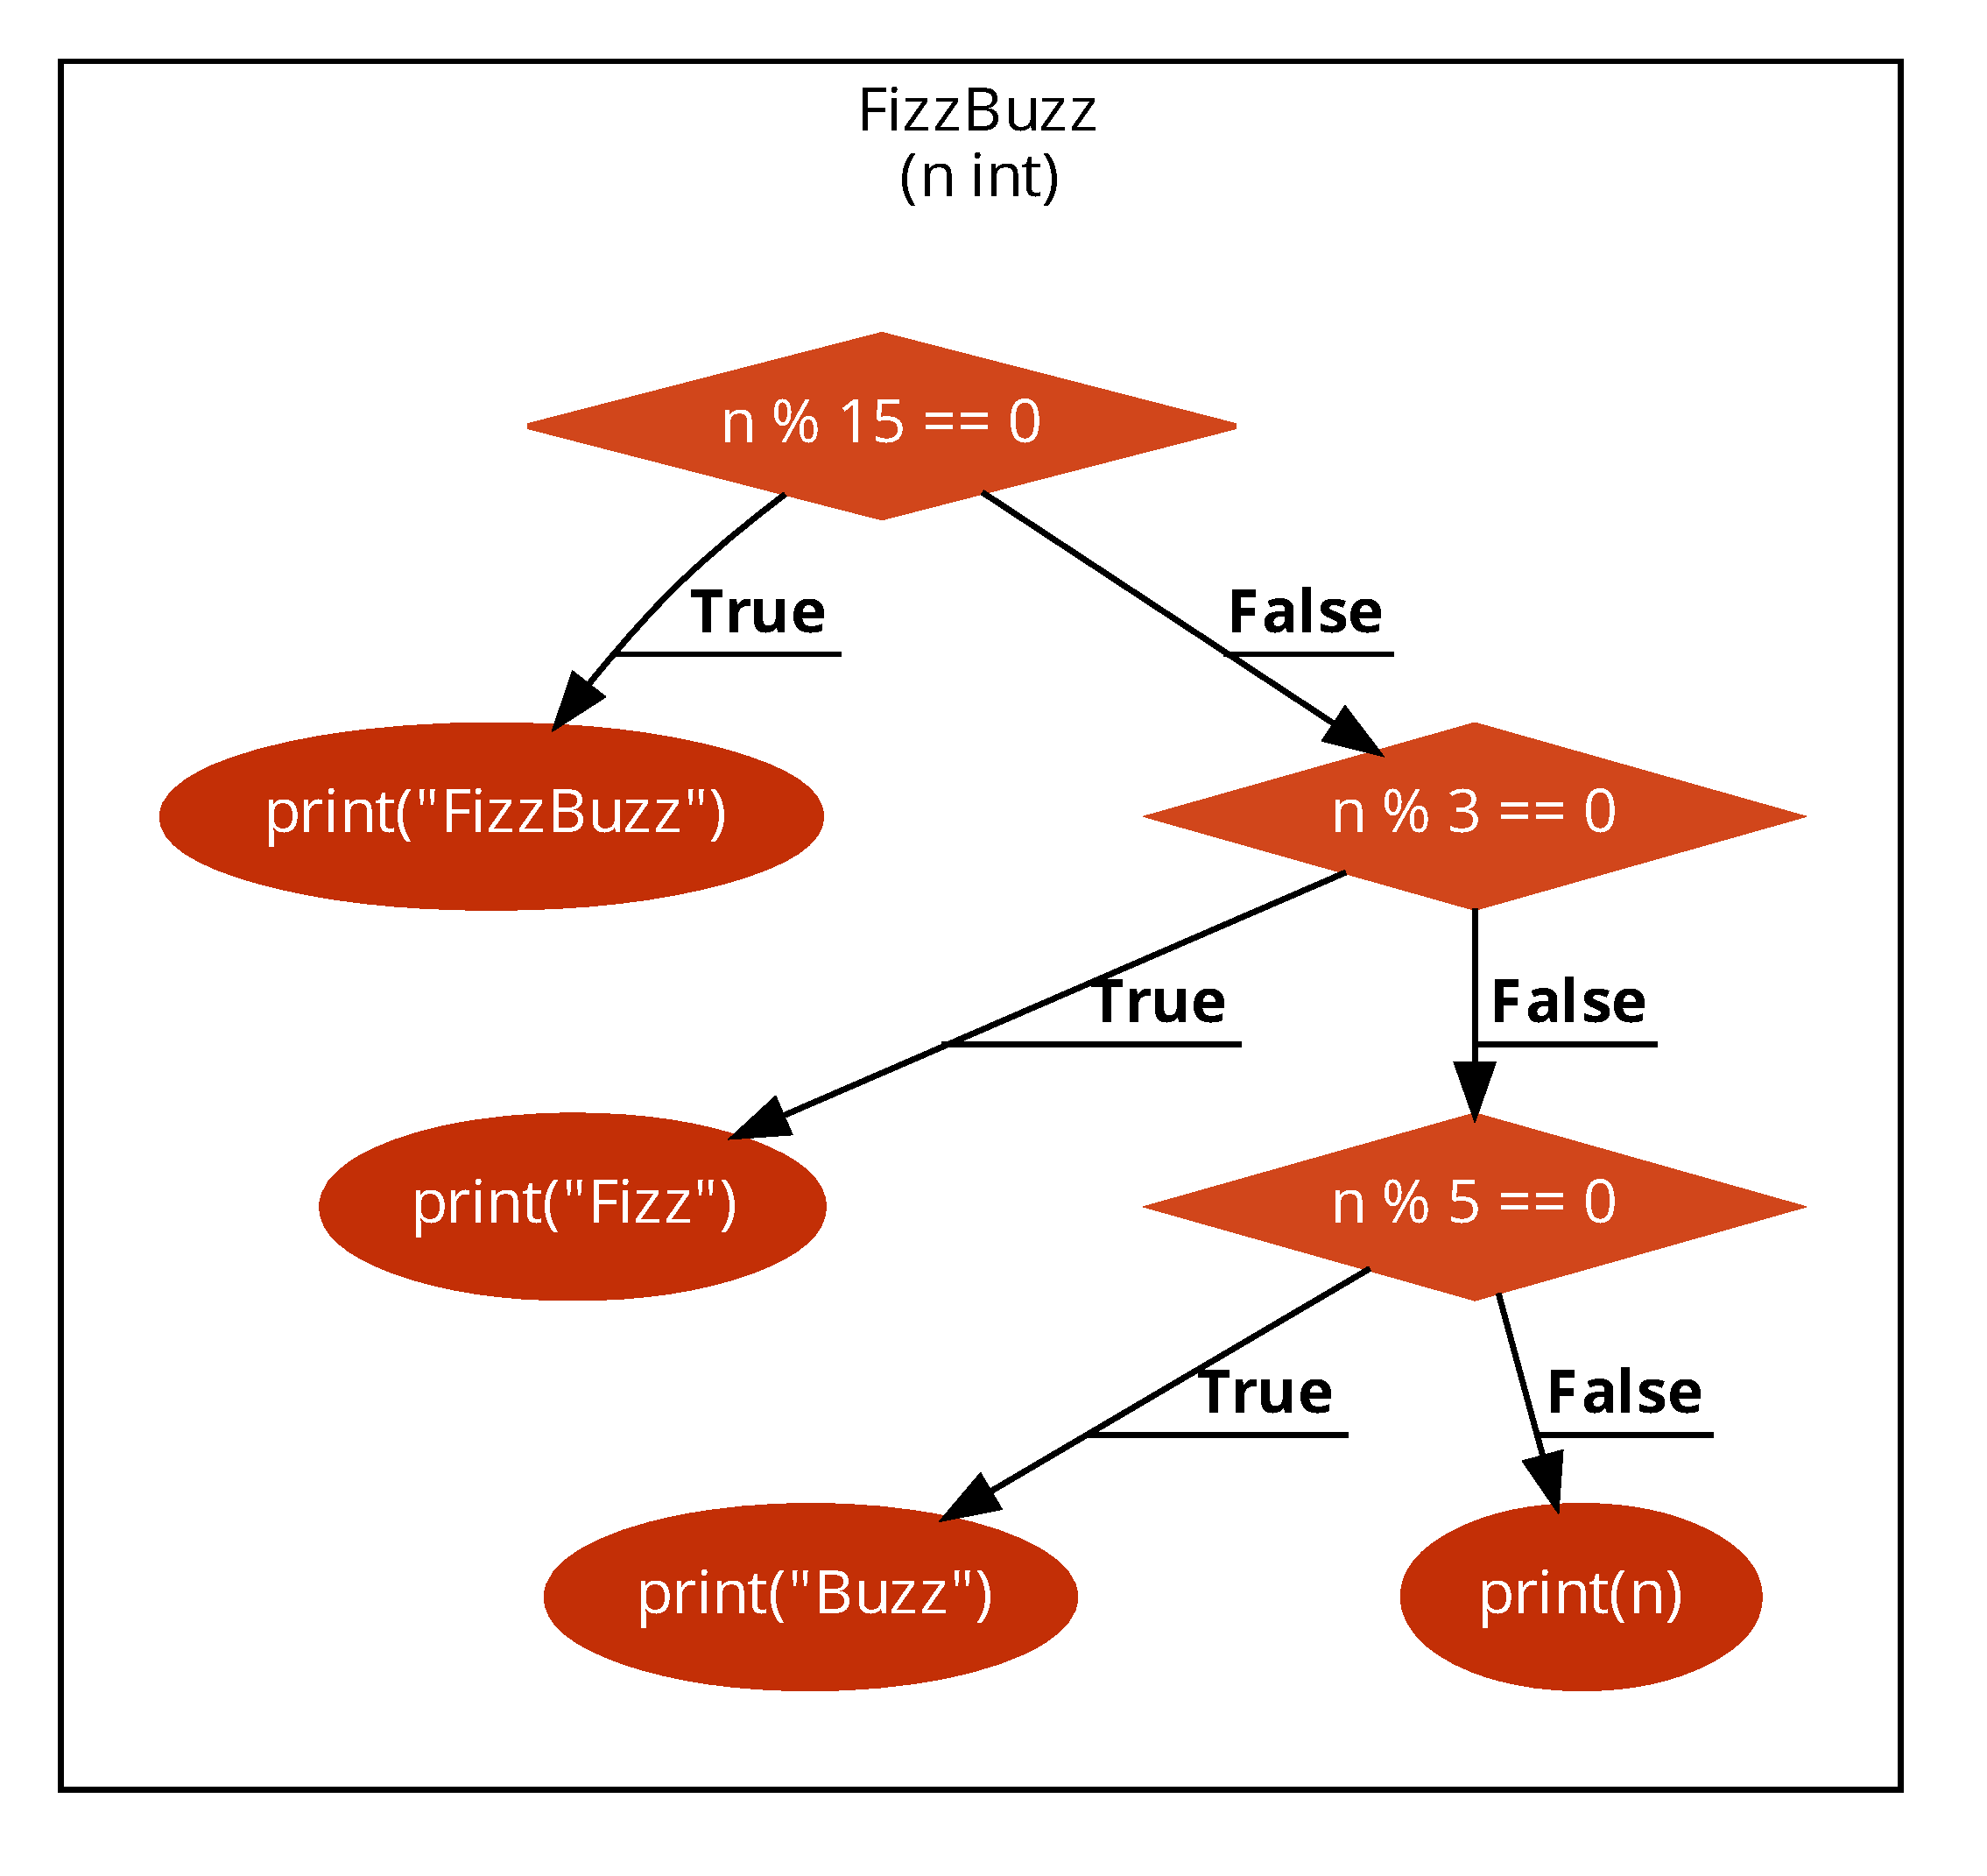
\includegraphics[scale=.2]{assets/chapter2/FizzBuzzCode2Flow.pdf}
   % \caption{The corresponding flowchart to \Cref{FizzBuzz written with Code2Flow.}.}
   % \label{The corresponding flowchart chapter2.}
%\end{figure}
